% !TeX program = pdflatex
% !TeX encoding = UTF-8
% !BIB program = biber
% paper_brm.tex -- Behavior Research Methods (original research article), English version.
% Translated from borrador_es.tex. APA 7 (apa7.cls) manuscript mode with double-blind masking
% ([mask] hides the author block; \blindtext hides the repository URLs). Tables and figures are
% generated by simulation/scripts/40_make_tables.R (TABLE_LANG=en -> tables_en/, figures *_en.pdf).
\documentclass[man,mask,donotrepeattitle,floatsintext]{apa7}

\usepackage[T1]{fontenc}
\usepackage[utf8]{inputenc}
\usepackage[american]{babel}
\usepackage{amsmath}
\usepackage{csquotes}
\usepackage[backend=biber,style=apa,sortcites=true,sorting=nyt]{biblatex}
\DeclareLanguageMapping{american}{american-apa}
\addbibresource{paper_brm.bib}
\graphicspath{{figures/}}

% Reuses apa7's own [mask] flag to also blind identifying URLs in the body text.
% #1 = real content (shown once [mask] is removed); #2 = placeholder shown during blind review.
\makeatletter
\newcommand{\blindtext}[2]{\@ifundefined{apaSeven@maskauthoridentity}{#1}{#2}}
\makeatother

\title{When Does Chatterjee's $\xi$ Work with Psychological Data, and When Does It Not? A Simulation and Real-Data Guide}
\shorttitle{Chatterjee's $\xi$ in Psychological Data}

\authorsnames{Arquímedes Chacón}
\authorsaffiliations{Universidad Católica Andrés Bello, Caracas, Venezuela}
\authornote{Correspondence concerning this article should be addressed to Arquímedes Chacón, Universidad Católica Andrés Bello, Caracas, Venezuela. Email: arquimedeschacon@gmail.com}

\leftheader{Chacón}

\abstract{Chatterjee's (2021) $\xi$ coefficient promises to detect any functional dependence between two variables with a simple asymptotic test, which makes it attractive for psychology, where non-monotonic relationships (inverted U and U shapes) are common. Its behavior with typical psychological data---ordinal or binary variables with ties, moderate samples, weak effects---is unknown. This article evaluates it in three reproducible studies. Study 1 examines by simulation the Type I error and power of its test with binary, ordinal, and composite-score responses. Study 2 compares it with Spearman's and Pearson's coefficients, distance correlation (dCor), and $\tau^*$ across four dependence structures calibrated by explained variance, with sample sizes from 50 to 800. Study 3 analyzes exhaustively 645 variable pairs from three public datasets (\texttt{bfi}, \texttt{sat.act}, and NHANES 2017--2018). The tie-aware $\xi$ test keeps its nominal level, except with highly unbalanced binary responses, where it is anticonservative; the version that assumes continuous variables fails with discrete responses. $\xi$ is by far the most powerful measure for oscillatory relationships, but it needs about eight times more participants than Spearman's coefficient for monotonic relationships and, in the real data, it never detected an association that Spearman's and Pearson's coefficients missed; dCor and $\tau^*$ did reveal non-monotonic associations, such as the U shape between sleep and depression. Moreover, with Likert-type items $\xi$ varies with the random tie-breaking as much as its own size. A practical guide is offered, and all code and results are public.}

\keywords{Chatterjee's coefficient, non-monotonic dependence, ties, ordinal data, Monte Carlo simulation, distance correlation}

\begin{document}
\maketitle

\section{Introduction}

Many psychological theories predict relationships that are not monotonic. The Yerkes--Dodson law \parencite{yerkes1908} holds that performance improves with arousal up to an optimal level and worsens afterward; the organizational behavior literature describes the ``too-much-of-a-good-thing'' effect, whereby beneficial traits or behaviors cease to be so at high levels \parencite{pierce2013}; and in mental health both short and long sleep are associated with a higher risk of depression \parencite{zhai2015}. Yet the coefficients that dominate practice---Pearson's and Spearman's correlations---measure linear or monotonic association and can be close to zero even when one variable is an exact function of the other, if that function is not monotonic \parencite{chatterjee2021}. A researcher who relies on them alone may conclude that ``there is no relationship'' where there is one.

Measures that detect general dependencies exist. Distance correlation (dCor; \cite{szekely2007}) and the $\tau^*$ coefficient of \textcite{bergsma2014} are zero only under independence, but their tests are computationally more costly (permutation, in the case of dCor). The $\xi_n$ coefficient of \textcite{chatterjee2021} is a recent proposal with attractive advantages for data analysts: it is computed from ranks in $O(n\log n)$ time, it is zero only under independence and one only if $Y$ is a function of $X$, and its distribution under independence is asymptotically normal, so it offers an independence test without resampling. Its appearance has quickly generated a theoretical literature on conditional dependence \parencite{azadkia2021}, bias reduction \parencite{dalitz2024}, families of coefficients \parencite{gao2024}, detection thresholds \parencite{auddy2024}, and continuity \parencite{ansari2026,bucher2025}, and a standard implementation exists in R \parencite{chatterjee2023xicor}.

However, the theory and the published simulations on $\xi_n$ refer mostly to continuous variables, without ties, and to strong effects. Psychological data are usually something else: items with few ordered categories, binary variables, composite scores, samples of tens or hundreds of participants, and weak effects, in which one variable explains only a small percentage of the variance of the other. Two features of $\xi_n$ make ties matter in a special way. First, when there are ties in $X$, its definition requires ordering the tied observations at random, so the computed value is a random variable: two analysts with the same data can obtain different values. Second, when $Y$ has ties, the asymptotic variance of the statistic under independence depends on the distribution of $Y$ \parencite{chatterjee2021}, so a test that assumes a continuous $Y$ may not have the nominal level. Common practices add to this, such as dichotomizing continuous variables \parencite{maccallum2002} or treating ordinal scales as if they were continuous \parencite{liddell2018}.

As far as could be established, there is no systematic evaluation of the Type I error and power of $\xi_n$ with this kind of data, no comparison with the alternatives on a scale of dependence strength that favors no measure, and no exhaustive application to real psychological datasets. Without that evidence, researchers do not know when they can trust $\xi_n$, when another measure is preferable, or how to report it.

This article provides that evidence through three studies, all with public, reproducible code and results. Study 1 evaluates by simulation the level and power of the $\xi_n$ test when $X$ and $Y$ are binary, ordinal, or composite scores, with sample sizes from 50 to 1000. Study 2 compares $\xi_n$ with Spearman's and Pearson's coefficients, dCor, and $\tau^*$ across four dependence structures, calibrated according to the proportion of variance explained by the structure and not according to the scale of any coefficient. Study 3 applies the five measures to all variable pairs of three public datasets (645 pairs), with an analysis rule fixed in advance. The article concludes with a practical guide on when to use $\xi_n$, when to prefer another measure, and how to report it.

\section{Chatterjee's $\xi_n$ Coefficient and Its Competitors}

\subsection{Definition and Properties}

Let $(X_i,Y_i)$, $i=1,\dots,n$, be independent pairs. The pairs are ordered so that $X_{(1)}\le\dots\le X_{(n)}$ (ties in $X$ are broken at random), $r_i$ denotes the rank of $Y_{(i)}$ among all the $Y_j$, and $l_i$ the number of $j$ such that $Y_j\ge Y_{(i)}$. The coefficient is
\begin{equation}
\xi_n(X,Y) = 1 - \frac{n\sum_{i=1}^{n-1}|r_{i+1}-r_i|}{2\sum_{i=1}^{n} l_i\,(n-l_i)}.
\end{equation}
It converges almost surely to a population parameter $\xi(X,Y)\in[0,1]$ that is zero if and only if $X$ and $Y$ are independent and one if and only if $Y$ is a measurable function of $X$ \parencite{chatterjee2021}. Under independence and with a continuous $Y$, $\sqrt{n}\,\xi_n$ converges to a normal distribution with mean zero and variance $2/5$, which yields an asymptotic independence test that rejects for large values of $\xi_n$.

Two properties matter for what follows. First, $\xi_n$ is directional: $\xi_n(X,Y)\neq\xi_n(Y,X)$ in general, because it measures the extent to which $Y$ is a function of $X$ and not the other way around. Second, its finite-sample behavior has known limits: with a continuous $Y$ the maximum possible value is $(n-2)/(n+1)$, so with small $n$ it cannot approach one \parencite{dalitz2024}; the bootstrap does not work for this statistic \parencite{dalitz2024} and, in general, no meaningful confidence intervals of exact level exist \parencite{bucher2025}. For this reason this article reports hypothesis tests for $\xi_n$ but not confidence intervals.

\subsection{Ties, Discretization, and Composite Scores}

With discrete variables, the definition of $\xi_n$ forces two decisions. Ties in $X$ are resolved by ordering the tied observations at random, so $\xi_n$ is a randomized statistic and its value changes with each tie-break. Ties in $Y$ change the ranks $r_i$ and the counts $l_i$ and, with them, the asymptotic variance under independence, which is no longer $2/5$ but depends on the law of $Y$ \parencite{chatterjee2021}. The standard implementation \parencite{chatterjee2023xicor} estimates that variance from the data by default (argument \texttt{ties = TRUE}), whereas with \texttt{ties = FALSE} it uses the formula valid for a continuous $Y$. In this article the former is called the ``tie-aware test'' and the latter the ``naive test.'' A composite score---the average of several items---takes many more distinct values than a single item and therefore has fewer ties; in contrast, dichotomizing a continuous variable \parencite{maccallum2002} introduces the maximum possible number of ties.

\subsection{Competing Measures and How to Compare Them}

$\xi_n$ is compared with the measures in Table~\ref{tab:medidas}. They do not estimate the same population parameter or share a scale, so their magnitudes are not comparable with one another; instead, they are compared by the level and power of their tests, which are rejection probabilities under the same data-generating conditions. This also requires a criterion of dependence strength that favors no measure: Study 2 fixes it through the proportion of the variance of $Y$ attributable to the deterministic structure (the $R^2$ of the true function), and not through the value of any coefficient.

\begin{table}
\caption{Association Measures Compared}
\label{tab:medidas}
\begin{threeparttable}
\small
\begin{tabular}{llll}
\toprule
Measure & What it detects & Symmetric & Test used \\
\midrule
Pearson $r$ & Linear association & Yes & $t$ test on $r$ \\
Spearman $\rho$ & Monotonic association & Yes & $t$ test on $\rho$ \\
dCor & Any dependence & Yes & Permutation \\
$\tau^*$ & Any dependence & Yes & Asymptotic (automatic mode) \\
$\xi_n$ & Functional dependence of $Y$ on $X$ & No & Asymptotic, tie-aware \\
\bottomrule
\end{tabular}
\begin{tablenotes}[flushleft]
\small
\item \textit{Note.} dCor: distance correlation \parencite{szekely2007}; $\tau^*$: Bergsma--Dassios coefficient \parencite{bergsma2014}; $\xi_n$: Chatterjee's coefficient \parencite{chatterjee2021}. The tests are described in the method of each study.
\end{tablenotes}
\end{threeparttable}
\end{table}

\section{Study 1: Level and Power of the $\xi_n$ Test With Discrete Data}

\subsection{Method}

\paragraph{Data.} Continuous latent variables were generated, and the observed variables were obtained by cutting the latent variable at population cut points, so that the number of cases per category varies at random from one sample to the next, as in real data. $X$ was continuous, binary 50/50, or ordinal with 5 skewed categories (proportions .05, .10, .15, .30, and .40). $Y$ was continuous; binary with proportions 50/50, 80/20, 90/10, or 95/5; ordinal with 5 skewed categories; ordinal with 7 categories and a floor effect (.35, .25, .15, .10, .07, .05, and .03); or a composite score of 5 six-category items. Each item was obtained by cutting $\theta+\varepsilon_j$ at its sextiles, with $\theta$ the standardized latent trait and $\varepsilon_j\sim N(0,1)$, and the score is the average of the five items.

\paragraph{Level (Type I error).} The latent variables of $X$ and $Y$ were independent standard normals. 3 types of $X$, 8 of $Y$, and $n\in\{50,100,250,500,1000\}$ were combined (120 cells, 5000 replications each; Monte Carlo standard error $\approx .003$ at $\alpha=.05$). In each replication the tie-aware asymptotic test (\texttt{XICOR} 0.4.1; \cite{chatterjee2023xicor}) and the naive test were computed, with $\alpha=.05$ and $\alpha=.01$. The criterion was the liberal robustness band of \textcite{bradley1978}: rejection rates between .025 and .075 at $\alpha=.05$. In 24 cells ($X$ continuous or binary; $Y$ continuous, binary 90/10, binary 95/5, or ordinal with 7 categories; $n=100,250,500$; 1000 replications) a permutation test was also evaluated ($B=499$; $p=(1+\#\{\xi_n^*\ge\xi_n\})/(B+1)$, permuting $Y$ and re-breaking the ties of $X$).

\paragraph{Power.} $Y=f(X)+\sigma\varepsilon$ with $f(x)=x$ (linear), $x^2$ (quadratic), or $\sin(2\pi x)$ (sinusoidal), and $X$ and $\varepsilon$ standard normal. The noise level $\sigma$ was calibrated on the continuous latent variable, before discretizing, so that $\xi=.15$ in each structure. 3 structures, 3 types of $X$, 8 of $Y$, and 5 sample sizes were combined (360 cells, 2000 replications each).

\paragraph{Tie-breaking noise.} To quantify the variability due to random tie-breaking, earlier simulations of the project were used (\texttt{scripts/03\_h2b.R}, \texttt{05\_h2d.R}, and \texttt{06\_h2d\_kvarying.R}), with $n=100$, $\xi\approx .49$, and a linear relationship: 300 datasets with 20 tie-breaks each for a discretized $X$, and 1000 replications for the 10-item composite score (500 in the series by number of items).

\subsection{Results}

\paragraph{Level.} Table~\ref{tab:s1nivel} summarizes the Type I error. In 119 of the 120 cells the tie-aware test was within Bradley's band (range .043--.076; the only exception was continuous $X$, $Y$ 90/10, and $n=50$, at .076). With continuous responses, ordinal responses, and composite scores the level was adequate at all sample sizes. With highly unbalanced binary responses the test is anticonservative and the inflation does not disappear as $n$ increases: with 5\% in the minority category the rates ranged from .052 to .072 and were still .069 at $n=1000$ (about 50 cases in the minority category). In the tail the inflation is greater: at $\alpha=.01$ the rates were .018 (90/10) and .025 (95/5), nearly double and two and a half times the nominal level. The results did not depend on whether $X$ was discretized (the average rates by type of $Y$ differed by less than .005 across types of $X$).

The naive test, which assumes a continuous $Y$, rejected too often with discrete responses: average rates of .142 to .154 with binary responses (about three times the nominal level), .084 with the 5-category ordinal, and .073 with the 7-category one. It was adequate only with a continuous $Y$ and with the composite score (.053 and .051), which has many distinct values.

\begin{table}
\caption{Type I Error of the $\xi_n$ Test Under Independence, With Continuous $X$}
\label{tab:s1nivel}
\begin{threeparttable}
\small
\footnotesize\setlength{\tabcolsep}{3pt}
\begin{tabular}{lccccccc}
\toprule
 & \multicolumn{5}{c}{Tie-aware test, $\alpha = .05$} & Naive & Tie-aware \\
\cmidrule(lr){2-6}
Response $Y$ & $n=50$ & $n=100$ & $n=250$ & $n=500$ & $n=1000$ & $\alpha = .05$ & $\alpha = .01$ \\
\midrule
Continuous & .051 & .053 & .052 & .058 & .050 & .053 & .010 \\
Binary 50/50 & .057 & .058 & .048 & .049 & .047 & .152 & .010 \\
Binary 80/20 & .059 & .055 & .049 & .050 & .051 & .146 & .012 \\
Binary 90/10 & .076 & .060 & .050 & .050 & .061 & .154 & .018 \\
Binary 95/5 & .052 & .064 & .072 & .070 & .069 & .142 & .025 \\
Ordinal, 5 categories (skewed) & .050 & .056 & .052 & .049 & .050 & .084 & .012 \\
Ordinal, 7 categories (floor effect) & .045 & .047 & .050 & .054 & .049 & .073 & .009 \\
5-item composite & .052 & .047 & .052 & .048 & .051 & .051 & .009 \\
\bottomrule
\end{tabular}

\begin{tablenotes}[flushleft]
\small
\item \textit{Note.} Rejection rates (5000 replications per cell). The tie-aware test is the \texttt{XICOR} test with \texttt{ties = TRUE}; the naive test uses the variance valid for a continuous $Y$. The last two columns average the five sample sizes. With binary or ordinal $X$ the results were equivalent (differences smaller than .005).
\end{tablenotes}
\end{threeparttable}
\end{table}

\paragraph{Remedy: Permutation test.} In the 24 cells evaluated, the permutation test kept the level but was conservative with unbalanced binary responses (rates of .021 to .038 at $\alpha=.05$ and .010 or less at $\alpha=.01$), and behaved like the asymptotic test with continuous and ordinal responses (.037--.062 and .042--.056, respectively). It is therefore a safe alternative, at the cost of power, when the minority category is very small.

\paragraph{Power with discrete responses.} Discretizing $Y$ reduces power (Figure~\ref{fig:s1}). With a linear relationship and $n=100$, power with a continuous $Y$ was .725; with binary 50/50, .474; with binary 90/10, .309; with 5-category ordinal, .625; and with the composite score, .561. With $n=250$ the figures were .962, .812, .488, .921, and .888. The loss is very large with unbalanced binary responses and moderate with ordinal responses and composite scores, and it shrinks to less than .08 from $n=250$ on. The exception is the quadratic structure, in which a 90/10 response detected better than the continuous one at $n=100$ (.757 versus .697), possibly because the minority category concentrates the extreme values, where the curvature shows up.

\begin{figure}
\caption{Power of the $\xi_n$ Test by Type of Response}
\label{fig:s1}
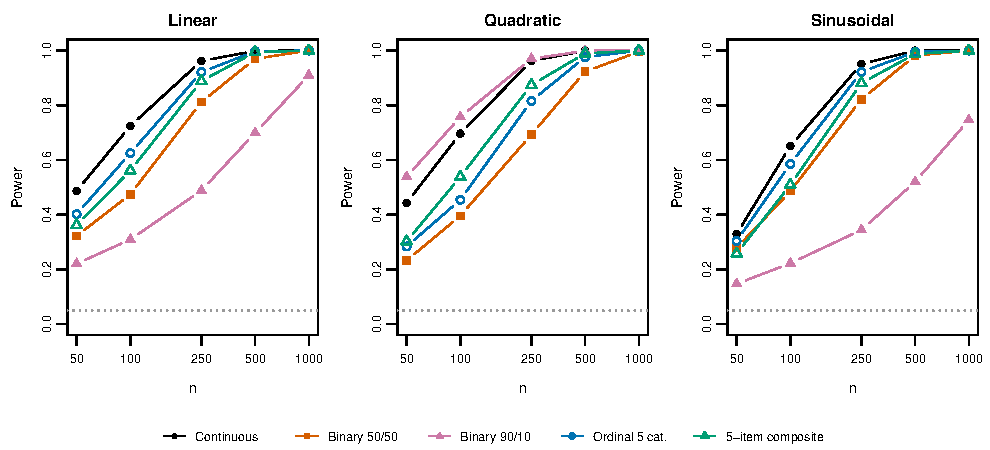
\includegraphics[width=\textwidth]{fig1_study1_en.pdf}
\figurenote{Power (2000 replications) with continuous $X$ and dependence calibrated to $\xi=.15$ on the latent variable. The dotted line marks the nominal level .05.}
\end{figure}

\paragraph{Discretizing the predictor.} Dichotomizing $X$ removes the ability of $\xi_n$ to detect non-monotonic relationships (Table~\ref{tab:s1x}). With $n=250$, power with a continuous $X$ was .962 (quadratic) and .951 (sinusoidal); with a binary 50/50 $X$ it was .052 and .056, that is, the nominal level; with a 5-category ordinal $X$, .602 and .182. With the linear structure, dichotomizing $X$ reduced power from .962 to .751.

\begin{table}
\caption{Power of $\xi_n$ by Discretization of $X$ (Continuous $Y$)}
\label{tab:s1x}
\begin{threeparttable}
\small
\footnotesize\setlength{\tabcolsep}{3pt}
\begin{tabular}{lcccccc}
\toprule
 & \multicolumn{3}{c}{$n = 100$} & \multicolumn{3}{c}{$n = 250$} \\
\cmidrule(lr){2-4}\cmidrule(lr){5-7}
Structure & Continuous & Binary 50/50 & Ordinal, 5 cat. & Continuous & Binary 50/50 & Ordinal, 5 cat. \\
\midrule
Linear & .725 & .431 & .591 & .962 & .751 & .917 \\
Quadratic & .697 & .055 & .324 & .962 & .052 & .602 \\
Sinusoidal & .651 & .062 & .110 & .951 & .056 & .182 \\
\bottomrule
\end{tabular}

\begin{tablenotes}[flushleft]
\small
\item \textit{Note.} Rejection rates at $\alpha=.05$ (2000 replications); dependence calibrated to $\xi=.15$ on the latent variable.
\end{tablenotes}
\end{threeparttable}
\end{table}

\paragraph{Tie-breaking noise.} When $X$ is discretized, part of the variability of $\xi_n$ does not come from the sample but from the random tie-breaking (Table~\ref{tab:s1tb}). With a binary $X$, 44\% of the total variability was due to tie-breaking alone, and the proportion decreased with more categories (37\%, 31\%, and 27\% with 3, 5, and 7 categories). A 10-item composite score reduced the empirical variance of $\xi_n$ by 37\% relative to a single item (from .0055 to .0035); the improvement leveled off from about 5 items (.0036) and was very small with up to 400 items (.0029).

\begin{table}
\caption{Variability of $\xi_n$ Between Datasets and Due to Random Tie-Breaking ($n=100$)}
\label{tab:s1tb}
\begin{threeparttable}
\small
\begin{tabular}{lccc}
\toprule
$X$ discretized into & Between datasets & Tie-breaking & \% tie-breaking \\
\midrule
Continuous & .0034 & .0000 & 0 \\
Binary & .0021 & .0017 & 44 \\
Likert-3 & .0022 & .0013 & 37 \\
Likert-5 & .0024 & .0011 & 31 \\
Likert-7 & .0026 & .0009 & 27 \\
\bottomrule
\end{tabular}

\begin{tablenotes}[flushleft]
\small
\item \textit{Note.} Variances of $\xi_n$ (linear relationship, $\xi\approx .49$; 300 datasets with 20 tie-breaks each). The last column is the share of the total variance due to tie-breaking.
\end{tablenotes}
\end{threeparttable}
\end{table}

\section{Study 2: $\xi_n$ Versus Competing Measures}

\subsection{Method}

\paragraph{Structures and neutral calibration.} The linear, quadratic, and sinusoidal structures of Study 1 were used, together with a circular structure: $X=2\Phi(Z)-1$, uniform on $(-1,1)$ with $Z$ standard normal, and $Y=S\sqrt{1-X^2}+\sigma\varepsilon$, with $S=\pm1$ with equal probability, so that $Y$ is not a function of $X$. The strength of dependence was set by the proportion of the variance of the latent $Y$ attributable to the deterministic structure, $R^2=\operatorname{Var}(f)/(\operatorname{Var}(f)+\sigma^2)$, that is, the $R^2$ of the true function, with $\operatorname{Var}(f)$ computed in a large noiseless sample. The same $R^2$ means the same amount of signal in the four structures, with no reference to the value of any coefficient. The values were .05, .13, .26, and .50 (.13 and .26 correspond to the medium and large effects of \textcite{cohen1988}) and, only for the circular structure, .70, .85, and .95, because with $R^2\le .50$ no test had appreciable power in that structure.

\paragraph{Responses and tests.} $X$ was continuous. $Y$ was continuous, binary 50/50, binary 90/10, ordinal with 5 skewed categories, or a composite score of 5 items (defined as in Study 1). The following were compared (Table~\ref{tab:medidas}): the tie-aware $\xi_n$ test; the $t$ tests of Spearman's and Pearson's coefficients; dCor with a permutation test ($B=199$; \texttt{energy} 1.7.12, \cite{rizzo2024energy}); and $\tau^*$ with the \texttt{TauStar} 1.1.9 test \parencite{weihs2026taustar}, which automatically chooses the continuous, mixed, or discrete mode according to the data. All tests were applied to the same simulated datasets.

\paragraph{Design.} Type I error: $n\in\{50,100,200,400\}$, 5 types of $Y$, 1000 replications. Power, with $\xi_n$, Spearman's, and Pearson's coefficients: 4 structures, 4 values of $R^2$, $n\in\{50,100,200,400,800\}$, and 5 types of $Y$, with 2000 replications. Power, with the five measures: $R^2\in\{.13,.26\}$ (and .70, .85, and .95 in the circular structure), $n\in\{50,100,200,400\}$, and $Y$ continuous, binary 50/50, ordinal, or composite, with 500 replications (standard error $\le .022$). The sample size needed for a power of .80 was interpolated log-linearly between the sizes evaluated. Because dCor and $\tau^*$ are costly, they were evaluated only up to $n=400$.

\subsection{Results}

\paragraph{Level.} The five tests kept the level (Table~\ref{tab:s2nivel}; .039 to .063 at $\alpha=.05$, averaging over $n$), except $\xi_n$ with $Y$ 90/10, which rejected .063 at $\alpha=.05$ and .018 at $\alpha=.01$, in line with Study 1. Spearman's and Pearson's coefficients, dCor, and $\tau^*$ did not show that problem (.052 to .057 with $Y$ 90/10). The $\tau^*$ routine issued numerical warnings in 24\% of the replications with $Y$ 90/10 (up to about 32\% in some cells) and in 5\% with a binary 50/50 $Y$, without its level being altered.

\begin{table}
\caption{Type I Error of the Five Tests Under Independence (Average Over $n=50$--$400$)}
\label{tab:s2nivel}
\begin{threeparttable}
\small
\begin{tabular}{lcccccc}
\toprule
Response $Y$ & $\xi_n$ & Spearman & Pearson & dCor & $\tau^*$ & $\tau^*$ warnings \\
\midrule
\multicolumn{7}{l}{\emph{Significance level .05}} \\
Continuous & .043 & .049 & .048 & .045 & .049 & 0\% \\
Binary 50/50 & .046 & .050 & .050 & .042 & .054 & 5\% \\
Binary 90/10 & .063 & .057 & .057 & .052 & .055 & 24\% \\
Ordinal, 5 categories (skewed) & .053 & .043 & .048 & .039 & .044 & 1\% \\
5-item composite & .049 & .053 & .051 & .049 & .053 & 0\% \\
\midrule
\multicolumn{7}{l}{\emph{Significance level .01}} \\
Continuous & .008 & .012 & .011 & .005 & .010 &  \\
Binary 50/50 & .009 & .011 & .011 & .006 & .012 &  \\
Binary 90/10 & .018 & .008 & .013 & .006 & .007 &  \\
Ordinal, 5 categories (skewed) & .009 & .008 & .006 & .004 & .007 &  \\
5-item composite & .009 & .010 & .009 & .005 & .011 &  \\
\bottomrule
\end{tabular}

\begin{tablenotes}[flushleft]
\small
\item \textit{Note.} Rejection rates (1000 replications per cell and sample size, continuous $X$). The last column is the proportion of replications in which the $\tau^*$ routine issued a numerical warning.
\end{tablenotes}
\end{threeparttable}
\end{table}

\paragraph{Power.} Figure~\ref{fig:s2} and Table~\ref{tab:s2n80} show that no measure dominates. In the \emph{linear} relationship, Pearson's and Spearman's coefficients are the most powerful and $\xi_n$ is much less powerful: with $R^2=.13$ and a continuous $Y$, 61 (Pearson) and 68 (Spearman) participants are needed for a power of .80, 74 and 75 with dCor and $\tau^*$, and 527 with $\xi_n$, about eight times more. In the \emph{quadratic} relationship, Pearson's and Spearman's coefficients detect nothing (power of .03 to .17 in the cells evaluated; $n_{80}>800$); the most powerful measure is dCor ($n_{80}=207$ with $R^2=.13$ and 98 with $R^2=.26$), followed by $\tau^*$ (314 and 156) and $\xi_n$ (685 and 206). In the \emph{sinusoidal} relationship, only $\xi_n$ reaches a power of .80 ($n_{80}=484$ with $R^2=.13$ and 136 with $R^2=.26$); with $R^2=.26$ and $n=400$ the power of dCor and $\tau^*$ was only .29 and .30, compared with .998 for $\xi_n$, and Spearman's and Pearson's coefficients did not exceed the nominal level. With ordinal responses the required sample sizes increase (for example, 647 versus 527 for $\xi_n$ with $R^2=.13$ in the linear relationship), but the ordering of the measures does not change.

\begin{figure}
\caption{Power of the Five Measures by Dependence Structure and Sample Size}
\label{fig:s2}
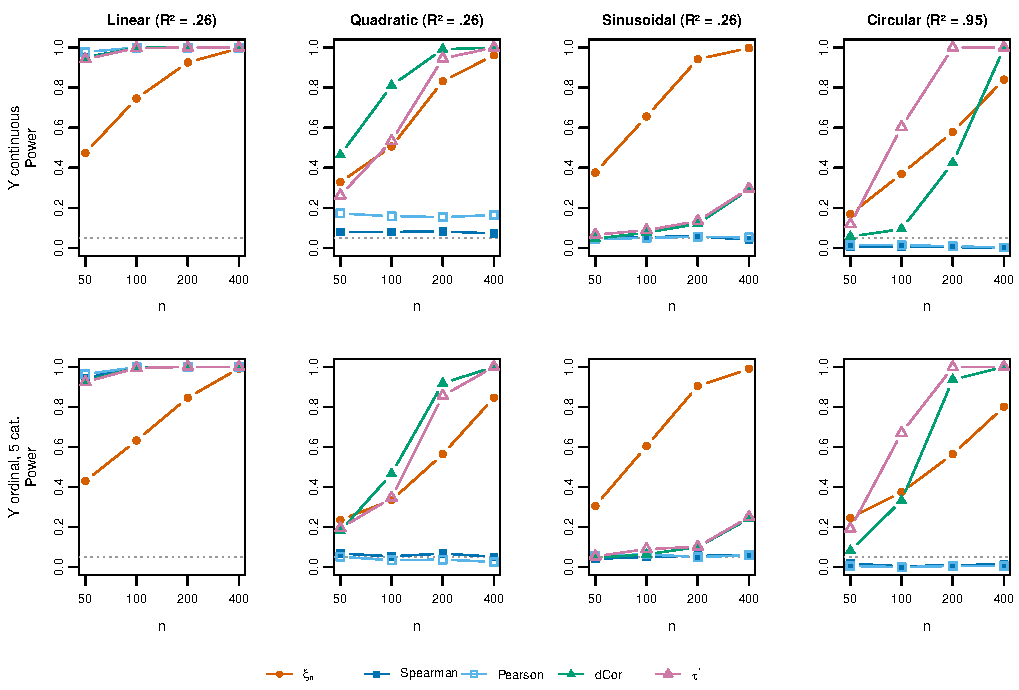
\includegraphics[width=\textwidth]{fig2_study2_en.pdf}
\figurenote{Power at $\alpha=.05$ (500 replications). $R^2=.26$ in the first three structures and $R^2=.95$ in the circular one. The dotted line marks the nominal level.}
\end{figure}

\begin{table}
\caption{Sample Size Needed for a Power of .80}
\label{tab:s2n80}
\begin{threeparttable}
\small
\setlength{\tabcolsep}{4pt}
\begin{tabular}{lllccccc}
\toprule
Structure & $R^2$ & Response $Y$ & $\xi_n$ & Spearman & Pearson & dCor & $\tau^*$ \\
\midrule
Linear & .13 & Continuous & 527 & 68 & 61 & 74 & 75 \\
 & .13 & Ordinal, 5 categories (skewed) & 647 & 75 & 72 & 81 & 82 \\
 & .26 & Continuous & 131 & $<$50 & $<$50 & $<$50 & $<$50 \\
 & .26 & Ordinal, 5 categories (skewed) & 162 & $<$50 & $<$50 & $<$50 & $<$50 \\
\addlinespace
Quadratic & .13 & Continuous & 685 & $>$800 & $>$800 & 207 & 314 \\
 & .13 & Ordinal, 5 categories (skewed) & $>$800 & $>$800 & $>$800 & 320 & 374 \\
 & .26 & Continuous & 206 & $>$800 & $>$800 & 98 & 156 \\
 & .26 & Ordinal, 5 categories (skewed) & 378 & $>$800 & $>$800 & 167 & 185 \\
\addlinespace
Sinusoidal & .13 & Continuous & 484 & $>$800 & $>$800 & $>$400 & $>$400 \\
 & .13 & Ordinal, 5 categories (skewed) & 606 & $>$800 & $>$800 & $>$400 & $>$400 \\
 & .26 & Continuous & 136 & $>$800 & $>$800 & $>$400 & $>$400 \\
 & .26 & Ordinal, 5 categories (skewed) & 157 & $>$800 & $>$800 & $>$400 & $>$400 \\
\bottomrule
\end{tabular}

\begin{tablenotes}[flushleft]
\small
\item \textit{Note.} Continuous $X$; $\alpha=.05$. Log-linear interpolation between the sizes evaluated. For $\xi_n$, Spearman's, and Pearson's coefficients, sizes up to $n=800$ were evaluated; for dCor and $\tau^*$, up to $n=400$.
\end{tablenotes}
\end{threeparttable}
\end{table}

In the \emph{circular} structure, with $R^2\le .50$ no measure exceeded a power of .10 even with $n=800$, so that range carries no information. With a strong signal (Table~\ref{tab:s2circ}), $\tau^*$ is the most powerful (with $R^2=.85$ and $n=200$: .474, versus .238 for $\xi_n$ and .176 for dCor; with $R^2=.95$ and $n=100$: .604, .370, and .094); $\xi_n$ outperforms dCor with $n\le 100$--$200$, but dCor outperforms it with $n=400$ (with $R^2=.95$: .998 versus .840); and Pearson's and Spearman's coefficients always fail (.022 or less). With a binary 50/50 response no measure exceeded a power of .07 in the circular structure.

\begin{table}
\caption{Power in the Circular Structure With a Strong Signal (Continuous $Y$)}
\label{tab:s2circ}
\begin{threeparttable}
\small
\begin{tabular}{llccccc}
\toprule
$R^2$ & $n$ & $\xi_n$ & Spearman & Pearson & dCor & $\tau^*$ \\
\midrule
.70 & 100 & .084 & .020 & .018 & .038 & .050 \\
 & 200 & .128 & .022 & .018 & .082 & .104 \\
 & 400 & .126 & .016 & .018 & .186 & .312 \\
.85 & 100 & .168 & .010 & .008 & .066 & .142 \\
 & 200 & .238 & .014 & .014 & .176 & .474 \\
 & 400 & .310 & .022 & .022 & .728 & .994 \\
.95 & 100 & .370 & .006 & .014 & .094 & .604 \\
 & 200 & .578 & .004 & .008 & .424 & 1.000 \\
 & 400 & .840 & .000 & .002 & .998 & 1.000 \\
\bottomrule
\end{tabular}

\begin{tablenotes}[flushleft]
\small
\item \textit{Note.} Rejection rates at $\alpha=.05$ (500 replications); $X$ uniform on $(-1,1)$.
\end{tablenotes}
\end{threeparttable}
\end{table}

\section{Study 3: Exhaustive Analysis of Real Data}

\subsection{Method}

\paragraph{Data and pairs.} Three public, freely accessible datasets were used. Two are in the R package \texttt{psych} \parencite{revelle2024psych}: \texttt{bfi} (2800 people, 25 six-category personality items from the SAPA project, plus gender, education, and age; \cite{revelle2010sapa}) and \texttt{sat.act} (700 students, with ACT, SAT verbal, SAT mathematics, age, gender, and education). The third is NHANES 2017--2018 \parencite{nhanes2017}, whose public-use files are downloaded without registration from the website of the U.S. Centers for Disease Control and Prevention (CDC) (\texttt{DEMO\_J}, \texttt{DPQ\_J}, \texttt{SLQ\_J}, and \texttt{BMX\_J}; the size and checksum of each file are recorded in the results). \emph{Every} pair of variables from a set fixed in advance was analyzed: in \texttt{bfi}, the 25 items, the 5 Big Five personality composite scores (item averages with the usual reverse coding), gender, education, and age (503 pairs after excluding item--own-composite pairs); in \texttt{sat.act}, its 6 variables (15 pairs); and in NHANES, adults aged 18 or older and 17 variables (the nine PHQ-9 items \parencite{kroenke2001} and their total, weekday and weekend sleep hours, age, gender, body-mass index, income-to-poverty ratio, and education; 127 pairs, excluding item--total pairs). Each pair used its complete cases. The NHANES analysis does not incorporate the survey sampling weights, so it describes the sample and not the U.S. population. The U shape between sleep hours and depression was expected from the literature \parencite{zhai2015}; nevertheless, to verify that the files were read correctly, the PHQ-9 means by bands of sleep hours, body-mass index, and age were inspected beforehand, so the choice of that dataset is not independent of that inspection. Even so, it is one of the 127 pairs, and all were analyzed with the same rule.

\paragraph{Measures and decision rule.} For each pair the following were computed: $\xi_n(X,Y)$ and $\xi_n(Y,X)$, averaged over 20 random tie-breaks, with their standard deviation across tie-breaks and the tie-aware asymptotic test (median of the $p$ values of the 20 tie-breaks); Spearman's and Pearson's coefficients, with a $t$ test and a confidence interval (for Spearman, with the variance $1.06/(n-3)$ of \cite{fieller1957}); dCor with a permutation test ($B=499$; the smallest attainable $p$ is .002); and $\tau^*$ with its test. No confidence intervals are computed for $\xi_n$ (see the Background section). A measure \emph{detects} an association in a pair if its $p$ value, adjusted by the Benjamini--Hochberg procedure \parencite{benjamini1995} within each dataset and measure, is less than .05; the $p$ value of $\xi_n$ is $\min\{1,2\min(p_{X\to Y},p_{Y\to X})\}$. This rule, the set of pairs, and the seeds were fixed before the analyses were run.

\subsection{Results}

\paragraph{Detection.} Table~\ref{tab:s3det} shows how many pairs each measure detects. $\xi_n$ detects far fewer than the others: in \texttt{bfi}, 138 of 503 pairs, versus 434 for Spearman, 428 for Pearson, 475 for dCor, and 477 for $\tau^*$; in NHANES, 42 of 127, versus 96, 97, 119, and 113. Moreover, in none of the 645 pairs did $\xi_n$ detect an association that Spearman's and Pearson's coefficients did not detect. There were, in contrast, pairs detected only by the general measures (40 in \texttt{bfi}, 20 in NHANES, and 1 in \texttt{sat.act}), always thanks to dCor or $\tau^*$; and in 296 pairs of \texttt{bfi} and 54 of NHANES, Spearman's coefficient detected an association that $\xi_n$ did not.

\begin{table}
\caption{Variable Pairs in Which Each Measure Detects an Association}
\label{tab:s3det}
\begin{threeparttable}
\small
\begin{tabular}{lccc}
\toprule
 & \texttt{bfi} & NHANES & \texttt{sat.act} \\
\midrule
Pairs analyzed & 503 & 127 & 15 \\
\midrule
\multicolumn{4}{l}{\emph{Pairs detected by each measure}} \\
Spearman & 434 & 96 & 8 \\
Pearson & 428 & 97 & 8 \\
$\xi_n$ & 138 & 42 & 4 \\
dCor & 475 & 119 & 10 \\
$\tau^*$ & 477 & 113 & 10 \\
\midrule
Only by general measures ($\xi_n$, dCor or $\tau^*$) & 40 & 20 & 1 \\
Only by Spearman or Pearson & 1 & 0 & 0 \\
$\xi_n$ detects and Spearman and Pearson do not & 0 & 0 & 0 \\
\bottomrule
\end{tabular}

\begin{tablenotes}[flushleft]
\small
\item \textit{Note.} Detection: Benjamini--Hochberg-adjusted $p$ value below .05, within each dataset and measure. The general measures are $\xi_n$, dCor, and $\tau^*$.
\end{tablenotes}
\end{threeparttable}
\end{table}

\paragraph{A case in which the conclusion depends on the measure.} With 5032 NHANES adults, the relationship between weekday sleep hours and depression (total PHQ-9) has a U shape (Figure~\ref{fig:s3}a): the mean PHQ-9 is 5.1 with fewer than 5 hours of sleep, about 2.9 with 7 to 9 hours, and 4.3 with 10 hours or more. Spearman's and Pearson's coefficients give $-.017$ ($p=.227$ and $.219$), so they would conclude that there is no relationship (Table~\ref{tab:s3nh}). $\xi_n$ does not detect it either ($p=.254$), but dCor ($p=.002$) and $\tau^*$ ($p<.001$) do. The relationship of body-mass index with depression also has a U shape (Figure~\ref{fig:s3}b); Spearman's coefficient detects it ($\rho=.102$, $p<.001$), but $\xi_n$ does not ($p=.268$).

\begin{figure}
\caption{Depression (Total PHQ-9) by Sleep Hours and Body-Mass Index}
\label{fig:s3}
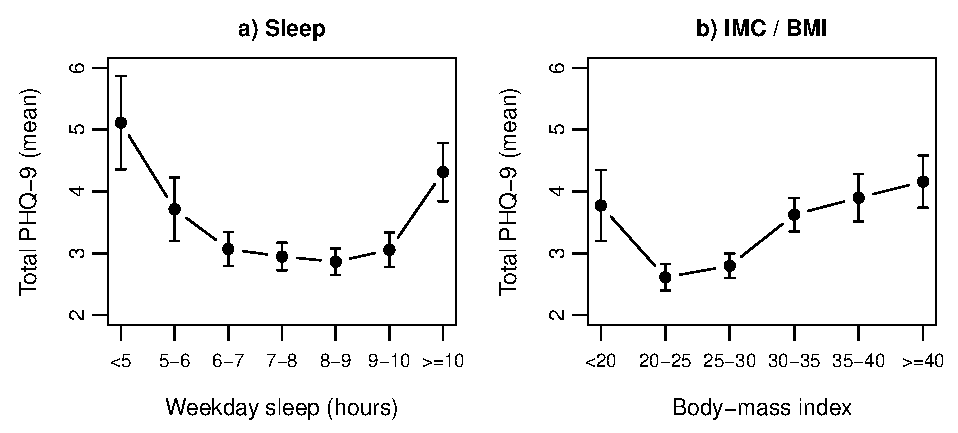
\includegraphics[width=\textwidth]{fig3_nhanes_en.pdf}
\figurenote{Means and 95\% confidence intervals by category, NHANES 2017--2018 adults (without sampling weights).}
\end{figure}

\begin{table}
\caption{Measures of Association Between Depression (Total PHQ-9) and Other Variables in NHANES}
\label{tab:s3nh}
\begin{threeparttable}
\small
\setlength{\tabcolsep}{4pt}
\begin{tabular}{lrcccc}
\toprule
Variable (vs. total PHQ-9) & $n$ & Spearman $\rho$ ($p$) & $\xi_n$ ($p$) & dCor ($p$) & $\tau^*$ ($p$) \\
\midrule
Weekday sleep (h) & 5032 & $-$.017 (.227) & .008 (.254) & .073 (.002)$^{\dagger}$ & .0009 ($<$ .001)$^{\dagger}$ \\
Weekend sleep (h) & 5026 & $-$.029 (.042) & .011 (.357) & .074 (.002)$^{\dagger}$ & .0010 ($<$ .001)$^{\dagger}$ \\
Body-mass index & 5010 & .102 ($<$ .001)$^{\dagger}$ & .012 (.268) & .117 (.002)$^{\dagger}$ & .0044 ($<$ .001)$^{\dagger}$ \\
Age & 5068 & $-$.040 (.004)$^{\dagger}$ & .004 (.706) & .038 (.010)$^{\dagger}$ & .0008 ($<$ .001)$^{\dagger}$ \\
Income-to-poverty ratio & 4438 & $-$.170 ($<$ .001)$^{\dagger}$ & .024 (.017) & .177 (.002)$^{\dagger}$ & .0101 ($<$ .001)$^{\dagger}$ \\
Gender & 5068 & .138 ($<$ .001)$^{\dagger}$ & .019 (.180) & .123 (.002)$^{\dagger}$ & .0055 ($<$ .001)$^{\dagger}$ \\
\bottomrule
\end{tabular}

\begin{tablenotes}[flushleft]
\small
\item \textit{Note.} In parentheses, the (unadjusted) $p$ value. For $\xi_n$, the larger of the two directions and the combined $p$ are shown. $^{\dagger}$ Detects the association according to the Benjamini--Hochberg-adjusted rule. $p=.002$ is the smallest value attainable with 499 permutations.
\end{tablenotes}
\end{threeparttable}
\end{table}

\paragraph{Tie-breaking noise.} With items of few categories, the value of $\xi_n$ changes with the random tie-breaking as much as its own size (Table~\ref{tab:s3tb}): the standard deviation of $\xi_n$ across tie-breaks had a median of .0139 in \texttt{bfi} and .0120 in NHANES, compared with medians of $|\xi_n|$ of .0167 and .0125. In 40\% of the \texttt{bfi} pairs and 24\% of the NHANES pairs, the $\xi_n$ test rejected independence (at $\alpha=.05$) in between 25\% and 75\% of the tie-breaks; that is, its decision depended on the chance of the tie-break, in at least one direction.

\begin{table}
\caption{Variability of $\xi_n$ Across Random Tie-Breaks in the Real Data}
\label{tab:s3tb}
\begin{threeparttable}
\small
\begin{tabular}{lcccc}
\toprule
 & Pairs & SD of $\xi_n$ across tie-breaks (median) & $|\xi_n|$ (median) & Unstable decision (\%) \\
\midrule
\texttt{bfi} & 503 & .0139 & .0167 & 40 \\
NHANES & 127 & .0120 & .0125 & 24 \\
\texttt{sat.act} & 15 & .0264 & .0207 & 20 \\
\bottomrule
\end{tabular}

\begin{tablenotes}[flushleft]
\small
\item \textit{Note.} Medians across pairs of the larger of the two directions. Unstable decision: the $\xi_n$ test changed its decision (at $\alpha=.05$) in between 25\% and 75\% of the 20 tie-breaks, in at least one direction.
\end{tablenotes}
\end{threeparttable}
\end{table}

\section{Discussion}

\subsection{What Was Found}

The three studies give a coherent picture. First, the $\xi_n$ test is valid under the usual conditions of psychological data---continuous and ordinal responses, composite scores, and balanced binary responses---as long as the tie-aware version is used; the version that assumes continuous variables rejects three times as often as it should with binary responses. It becomes anticonservative with highly unbalanced binary responses (5 to 10\% in one category), especially in the tail, and the problem does not disappear with large sample sizes. Second, $\xi_n$ is by far the most powerful measure for oscillatory relationships, but it is much less powerful than the others for monotonic relationships and, with small effects such as those in psychology, for U shapes: dCor and $\tau^*$ are preferable for the latter. Third, in the real data $\xi_n$ never detected anything that Spearman's and Pearson's coefficients overlooked; the associations that these missed---such as the U shape between sleep and depression---were detected by dCor and $\tau^*$. Fourth, with items of few categories the value of $\xi_n$ is dominated by the random tie-breaking, and dichotomizing $X$ with a median split eliminates the signal of symmetric non-monotonic relationships, so that $\xi_n$ falls to the nominal level.

\subsection{Practical Guide}

Table~\ref{tab:guia} summarizes which measure to use according to the type of relationship suspected. In addition, the following is recommended when reporting $\xi_n$: (a) use the tie-aware test (in \texttt{XICOR}, \texttt{ties = TRUE}, the default) and not the one that assumes continuous variables; (b) state the direction of the coefficient, $\xi_n(X,Y)$ or $\xi_n(Y,X)$; (c) when there are ties, average $\xi_n$ over several tie-breaks (here, 20) and report its standard deviation, rather than a single value; (d) with a binary response whose minority category is smaller than about 5\% (or about 50 cases), report the number of cases in that category and prefer the permutation test; (e) do not report bootstrap confidence intervals for $\xi_n$; and (f) do not dichotomize continuous variables before the analysis. Composite scores posed no problems.

\begin{table}
\caption{Guide to Choosing an Association Measure According to the Expected Relationship}
\label{tab:guia}
\begin{threeparttable}
\small
\begin{tabular}{p{3.6cm}p{4.2cm}p{6.6cm}}
\toprule
Expected relationship & Recommended measure & Caveat \\
\midrule
Linear or monotonic & Pearson or Spearman & $\xi_n$ needs about eight times more participants for the same power ($R^2=.13$). \\
U shape or inverted U & dCor or $\tau^*$ (in this study, dCor was the most powerful); $\xi_n$ as a complement & Pearson and Spearman can be near zero (sleep and depression: $\rho=-.017$). \\
Oscillatory or complex functional & $\xi_n$ & It is the only one that reaches a power of .80 with $n\le 400$ ($n\approx 140$ with $R^2=.26$). \\
Non-functional (e.g., circular) & $\tau^*$; dCor with large $n$ & $\xi_n$ is intermediate; no measure detects weak signals ($R^2<.70$). \\
Exploring many pairs with weak effects & Spearman together with dCor or $\tau^*$; plot the pairs detected only by the general measures & $\xi_n$ detected fewer pairs than Spearman (138 versus 434 in \texttt{bfi}). \\
\bottomrule
\end{tabular}
\begin{tablenotes}[flushleft]
\small
\item \textit{Note.} Based on Studies 1 to 3; the figures correspond to the simulated conditions.
\end{tablenotes}
\end{threeparttable}
\end{table}

\subsection{Limitations}

The simulations use normal latent variables, four dependence structures, one dependence at a time, and a single explanatory variable; other distributions or shapes could change the required sample sizes. Calibration by explained variance is one of several possible scales, and the one chosen is not useful for structures whose signal lies in the conditional variance. Permutation tests have limited resolution (with 499 permutations the smallest $p$ is .002), and the power results with the five measures are based on 500 replications, so differences smaller than about .04 should not be interpreted. In the real data, the fact that dCor or $\tau^*$ detect a pair that Spearman's coefficient does not detect does not by itself demonstrate a non-monotonic shape: with samples of thousands of people even very small dependencies become significant, and significance is not the same as practical relevance; in this article only the shape of the sleep and body-mass index pairs was checked graphically. The NHANES analysis does not use sampling weights. Finally, $\xi_n$ was evaluated only in its bivariate version and without confidence intervals, for the reasons given.

\subsection{Open Science}

All the code (data generation, tests, analyses, tables, and figures) and the raw results are available in a public repository; the simulations and the real-data analyses were run with GitHub Actions workflows with fixed seeds, and two independent runs of the main blocks of Study 2 produced byte-identical files.

\section*{Declarations}

\paragraph{Funding.} This work received no specific funding.

\paragraph{Conflicts of interest.} The author declares no conflicts of interest.

\paragraph{Ethics approval and consent.} Not applicable: the study uses simulated data and public secondary data without identifiable information.

\paragraph{Availability of data and materials.} The \texttt{bfi} and \texttt{sat.act} data are in the CRAN package \texttt{psych} (\texttt{data(bfi, package = "psych")}; \texttt{data(sat.act, package = "psych")}). The NHANES 2017--2018 files (\texttt{DEMO\_J}, \texttt{DPQ\_J}, \texttt{SLQ\_J}, \texttt{BMX\_J}) are downloaded without registration from \url{https://wwwn.cdc.gov/Nchs/Data/Nhanes/Public/2017/DataFiles/}, and their size and checksum are recorded in the results. The raw results of the simulations and of the real-data analyses are at \blindtext{\url{https://github.com/ArchieJamDev/ChatterjeeXi-Simulation}}{[anonymous link for review]}.

\paragraph{Code availability.} All the code is in the same repository (\blindtext{\url{https://github.com/ArchieJamDev/ChatterjeeXi-Simulation}}{[anonymous link for review]}), with execution instructions, fixed seeds, and the GitHub Actions workflows with which the results were produced. Software: R \parencite{rcore2025}, \texttt{XICOR}, \texttt{energy}, \texttt{TauStar}, and \texttt{psych}.

\paragraph{Author contributions.} Sole author: conception, design, analysis, writing.

\paragraph{Use of artificial intelligence tools.} An artificial intelligence assistant (Claude, Anthropic) was used as support to run and verify the simulations and to assist in developing the necessary code. The author designed, developed, reviewed, and verified the code, the results, and the text, and is solely responsible for the content.

\section*{Open Practices Statement}

The data and code of this study are publicly available (see Availability of data and materials and Code availability). No part of the study was preregistered; the analysis rule of Study 3 (set of pairs, measures, and decision criterion) was fixed in the code before the analyses were run, and the repository history documents it.

\printbibliography

\end{document}
